\graphicspath{ {images/} }
\chapter{Literature Review}
%\subsection*{}
%\textbf{[1]}\\
\hspace{5mm} Research has been done to provide security framework for BYOD paradigm for employees and organisation.BYOD security framework proposed and prototyped using Mobile Device Management (MDM) but still industries not satisfied with security policies(due  to inside and outside threat).
Because of this reason ,BYOD security still in research.

\section{Survey Existing system} 
A security framework for mobile devices that ensures that only applications that comply with the organization security policy are installed on the registered devices in which the framework consists of 1) a security policy manager that mediates access to the applications stores by (i) keeping track of the security state of the registered devices and (ii) determining whether an application can be safely added to a device and
2) An installer application that tells the user which applications can be safely installed, which need further scrutiny by the security policy manager and finally which are known to violate the security policy~\cite{aless,sean}, paper author present a type and effect system which allows us to infer history expressions from application implementations.

\par presented analysis report on impact on fast growing trend in mobile market where analysis report contains consumerisation(personal devices are used for work as well as leisure) benefits for the Enterprise,Consumerization concerns,auther explained about consumerisation trends,spread if BYOD,consumerisation benefits for the enterprise(BYOD appeals to the enterprise finance managers, where users pay for their own devices and the internal application farm is replaced by free web services),consumerization concerns(Small and light portable devices can be lost or stolen easily, and with them - confidential corporate data and access to enterprise facilities)~\cite{ben}.

\par Paper cited above cover two models which can be used to manage the mobile devices in an organization to bring in BYOD~\cite{pra},i.e Mobile Device Management(MDM) and Cloud Architecture for Mobile Devices where the mobile device management tool helps the organization to fully control the devices which are generally supported by API`s of smartphones used and the MDM tool helps on the security and management of device by monitoring, controlling and protecting the device.
MDM architecture and BYOD concept control objectives
a) Identification and access control
b) Data protection
c) Application security
d) Integrity control
e) compliance

\par The paper selects major domestic and external web sites which provide cloud, VoIP, messenger, E-mail services and examines whether data are encrypted or not for constructing a safe Smart Work infrastructure,in which auther had explained about SSL/TLS (Definotion of SSL/TLS
,SSL/TLS Handshacking) which is the basis judgement of encryption of data,also auther explained about countermeasuresfor vulnerability,SSL modes~\cite{dae}.

\par BYOD security concerns and potential threats~\cite{den,ant} are define and targeted in different environment of access control and people in center,generally worked on data exfiltration,data tampering and data unavailibilty.

\par Formally define a subset of the existing se-
curity framework of Android, which suffices to define proposed extensions rigorously,also described the exten-
sions to the existing mechanism for incorporating usage constraints, and created a policy enforcement framework that incorporates usage policies while granting permissions to applications for accessing resources; and described and implemented an extended package installer that utilizes an easy-to-use and intuitive interface for allowing users to specify their constraints~\cite{apex}.


\section{Limitation Existing system or research gap}
\par (List them with  bullet points)The Cisco BYOD solution builds on the Cisco Border less Network architecture and assumes best practices are followed in network infrastructure designs for campus, branch offices, Internet edge, and home office implementations.
This comprehensive BYOD solution provided for wired, Wi-Fi, remote, and mobile access to the network, supporting across many device types and brands, and capable of enforcing the various policies across the spectrum of businesses and industries.
In addition, as devices move from one context to another, for example from the corporate WiFi network to a public 3G/4G mobile network, the BYOD solution provide secure access while keeping the experience seamless for the user.

\section{Problem Statement and objectives}
\par System is fully configured with network devices which nearly non affordable for small scale organization,where they always search for open source solution.Figure 2.1 describe high level architecture.
\subsection{Objectives}List objectives using bullet points
\section{Scope}
\par In addition, as devices move from one context to another, for example from the corporate WiFi network to a public 3G/4G mobile network, the BYOD solution provide secure access while keeping the experience seamless for the user.
\par example how to add image/figure
\begin{figure}[h!]
\begin{center}
\scalebox{0.75}{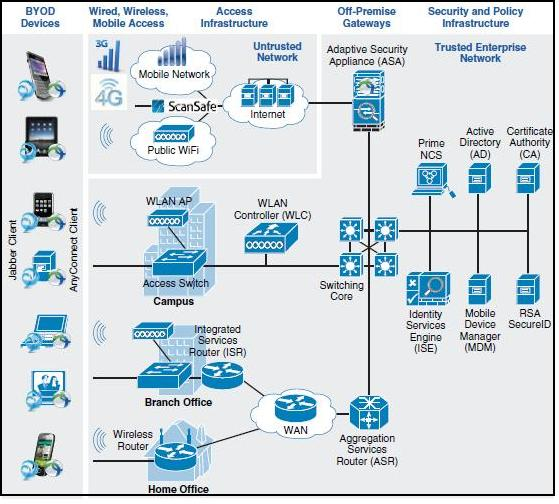
\includegraphics{CISCO-BYOD.jpeg}}
\end{center}
\caption {CISCO-High level BYOD Solution Architecture}
\label{vmb2}
\vspace{0mm}
\end{figure} 
  

